
\documentclass[12pt]{article} 

\usepackage{geometry}
\geometry{a4paper} 

\usepackage{graphicx} 
\usepackage{enumitem}
\usepackage{booktabs}

\usepackage{float} 
\usepackage{wrapfig} 

\usepackage{amsmath}
\usepackage{amsfonts}
\usepackage{amssymb}
\usepackage{dsfont}

\usepackage{hyperref} 


\usepackage{xcolor}
\usepackage{listings}
\usepackage{caption}
\DeclareCaptionFont{white}{\color{white}}
\DeclareCaptionFormat{listing}{%
  \parbox{\textwidth}{\colorbox{gray}{\parbox{\textwidth}{#1#2#3}}\vskip-2pt}}
\captionsetup[lstlisting]{format=listing,labelfont=white,textfont=white}
\lstset{frame=lrb,xleftmargin=\fboxsep,xrightmargin=-\fboxsep}

\linespread{1.2} 
\setlength{\parskip}{\baselineskip} % vertical spaces
\setlength\parindent{0pt} % remove all indentation from paragraphs



\begin{document}

\title{\textbf{Transformations, Diagnostics, \\ \& Polynomial Models}}
\author{Hyunwoo Gu}
\date{}

\maketitle



\section*{Contents}

\begin{itemize}
	\item Review of Multiple Regression : Orthogonal Case
	\item Transformations and Weighting to Correct Model Inadequacies 
	\item Diagnostics for Leverage and Influence
	\item Polynomial Regression Models
\end{itemize}


%----------------------------------------------------------------------------------------
% Section 5.1
%----------------------------------------------------------------------------------------
\section{Introduction}

This chapter focuses on methods and procedures for building regression models when some of the following assumptions are violated:

\begin{itemize}
  \item Errors $\overset{\text{uncorr}}{\sim} (0, \sigma^2_{\text{constant}})$ 
  \item Errors $\overset{iid}{\sim} Normal$
  \item The form of the model, including the specification of the regressors, is correct
\end{itemize}

\textbf{Data transformation} will be put emphasis on. Ideally, the choice of metric should be made by the engineer or scientist with \textbf{subject-matter knowledge}.

%----------------------------------------------------------------------------------------
% Section 5.2
%----------------------------------------------------------------------------------------
\section{Variance-stabilizing Transformations}

The assumption of \textbf{constant variance} is a basic requirement of regression analysis. It is important to detect and correct a nonconstant error variance. If this problem is not eliminated, the least-squares estimators will still be unbiased, but they will no longer have the minimum-variance property. 


\begin{table}[h!]
\begin{center}
\begin{tabular}{|c|c|}
\hline Relationship of $\sigma^2$ to $\mathbb{E}(y)$ & Transformation \\\hline
  $\sigma^2 \propto \mathrm{constant}$ & $y' = y$  \\
  $\sigma^2 \propto \mathbb{E}(y)$ & $y' = \sqrt{y}$  \\
  $\sigma^2 \propto [\mathbb{E}(y)][1-\mathbb{E}(y)]$ & $y' = \mathrm{sin}^{-1} \left( \sqrt(y)  \right)$  \\
  $\sigma^2 \propto [\mathbb{E}(y)]^2$ & $y' = \mathrm{ln} (y)$  \\
  $\sigma^2 \propto [\mathbb{E}(y)]^3$ & $y' = y^{-1/2}$  \\
  $\sigma^2 \propto [\mathbb{E}(y)]^4$ & $y' = y^{-1}$  \\\hline
\end{tabular}
\end{center}
\end{table}

The \textbf{strength} of a transformation depends on the amount of curvature that it induces. It is often necessary to convert the predicted values back to the original units. Unfortunately, applying the inverse transformation directly to the predicted values gives an estimate of the median of the distribution of the response instead of the mean.

%----------------------------------------------------------------------------------------
% Section 5.3
%----------------------------------------------------------------------------------------
\section{Transformations to Linearize the Model}

Nonlinearity may be detected via the lack-of-fit test or from scatter diagrams, the matrix of scatterplots, or residual plots such as the partial regression plot. In some cases a nonlinear function can be linearized by using a suitable transformation. Such nonlinear models are called \textbf{intrinsically} or \textbf{transformably linear}. 


\begin{table}[h!]
\begin{center}
\begin{tabular}{|c|c|c|c|}
\hline Figure & Linearizable Function & Transformation & Linear Form \\\hline
  \includegraphics[scale=0.3]{ab.png}
& $y = \beta_0 x^{\beta_1}$ & $y' = \mathrm{log} y, x' = \mathrm{log} x$ & $y' = \mathrm{log} \beta_0 + \beta_1 x'$ \\
  \includegraphics[scale=0.3]{cd.png}
& $y = \beta_0 e^{\beta-1x}$& $y' = \mathrm{log} y$                       & $y' = \mathrm{log} \beta_0 + \beta_1 x$ \\
  \includegraphics[scale=0.3]{ef.png} 
& $y = \beta_0 + \beta_1 \mathrm{log}x$ & $x' = \mathrm{log} x$            & $y' = \beta_0 + \beta_1 x'$ \\
  \includegraphics[scale=0.3]{gh.png}
& $y = \frac{x}{\beta_0x - \beta_1}$ &$y' = \frac{1}{y}, x' = \frac{1}{x}$ & $y' = \beta_0 - \beta_1 x'$ \\\hline
\end{tabular}
\end{center}
\end{table}


Consider the following exponential function, and a \textbf{logarithmic transformation}

$$
\begin{aligned}
y &= \beta_0 e^{\beta_1 x} \epsilon \\[10pt]
\mathrm{ln} y &= \mathrm{ln} \beta_0 + \beta_1 x + \mathrm{ln} \epsilon, \ \ \text{or}\\[8pt]
y' &= \beta_0' + \beta_1 x + \epsilon'
\end{aligned}
$$


BTW, various types of reciprocal transformations are also useful. For instance, the following model can be linearized by using the \textbf{reciprocal transformation} $x' = 1/x$. 

$$
\begin{aligned}
y &= \beta_0 + \beta_1 \left( \frac{1}{x} \right) + \epsilon \\[8pt]
y &= \beta_0 + \beta_1 x' + \epsilon \\[8pt]
\frac{1}{y} &= \beta_0 + \beta_1 x + \epsilon \\[8pt]
y &= \frac{x} {\beta_0 x - \beta_1 + \epsilon}
\end{aligned}
$$

When transformations such as those described above are employed, the least-squares estimator has \textbf{least-squares properties with respect to the transformed data}, not the original data.



%----------------------------------------------------------------------------------------
% Section 5.4
%----------------------------------------------------------------------------------------
\section{Analytical Methods for Selecting a Transformation}

\subsection{Transformations on $y$: The Box-Cox Method}

When we wish to transform $y$ to correct nonnormality and/or nonconstant variance, a useful class of transformations is the \textbf{power transformation} $y^\lambda$, where $\lambda$ is a parameter to be determined. 

To solve the problem of $y^\lambda$ approaching to unity when $\lambda \to 0$, one approach uses $(y^\lambda - 1)/\lambda$ as the response. Whilst solving the discontinuity problem, since $\lim_{\lambda \to 0} (y^\lambda - 1)/\lambda = \mathrm{log}(y)$, this is still a problem, since $(y^\lambda - 1)/\lambda$ change dramatically as $\lambda$ changes. 

The appropriate procedure is to use

$$
\begin{aligned}
y &= \begin{cases} \frac{y^\lambda - 1}{\lambda \dot{y}^{\lambda-1}}, & \lambda \neq 0 \\
                   \dot{y} \mathrm{ln}(y) \end{cases} \\[8pt]
y^{(\lambda)} &= X\beta + \epsilon
\end{aligned}
$$

where $\dot{y} := \mathrm{exp} [ 1/n \sum_i^n \mathrm{ln} (y_i) ]$ is the geometric mean of the observations. The divisor $\dot{y}^{\lambda - 1}$ is related to the \textbf{Jacobian} of the transformation,

$$
J(\lambda; y_1, \cdots, y_n) := \prod_i^n |dy_i^{(\lambda)}/dy| = \prod_i^n y_i^{\lambda-1} = [GM(y)]^{n(\lambda-1)}
$$

Thus, absorbing $GM(y)^{2(\lambda-1)}$ into the expression for $\hat{\sigma^2}$ produces an expression that establishes that minimizing the sum of squares of residuals from $y_i^{(\lambda)}$ is equivalent to maximizing the sum of the normal log likelihood of deviations from $(y^\lambda-1)/\lambda$ and the log of the Jacobian of the transformation.

$$
\begin{aligned}
l(\hat{\mu},\hat{\sigma^2}) &= \frac{-n}{2} \left(\mathrm{log}(2\pi\hat{\sigma}^2) + 1 \right) + n(\lambda-1)\mathrm{log}(GM(y)) \\[8pt]
&= \frac{-n}{2} \left(\mathrm{log}(2\pi\hat{\sigma}^2/GM(y)^{2(\lambda-1)}) + 1 \right)
\end{aligned}
$$


\subsubsection*{Computational Procedure}

The (profile) MLE of $\lambda$ corresponds to the value of $\lambda$ for which the residual sum of squares from the fitted model $SS_{Res}(\lambda)$ is a minimum. This value of $\lambda$ is usually determined by fitting a model to $y^{(\lambda)}$ for various values of $\lambda$, plotting the residual sum of squares $SS_{Res}(\lambda)$ versus $\lambda$.

Note that we \textbf{cannot} select $\lambda$ by \textbf{direct} comparison, since for each $\lambda$ the Residual SS is measured on a different scale. 



\subsubsection*{An Approximate Confidence Interval for $\lambda$}

An approximate CI for the transformation parameter $\lambda$ can be found, and this CI can be useful in selecting the final value for $\lambda$. 

In applying the \textbf{profile} maximum likelihood method to the regression model, we are essentially maximizing

$$
\begin{aligned}
L(\lambda) &= -\frac{n}{2} \mathrm{ln} (SS_{Res}(\lambda)) \\[8pt]
L(\hat{\lambda}) - L(\lambda) &\le \chi^2_\alpha(1)/{2n}
\end{aligned}
$$

If we are minimizing the residual sum of squares and plotting $SS_{res}(\lambda)$ versus $\lambda$, then the line must be plotted at height

$$
SS^\ast = SS_{Res}(\hat{\lambda}) e^{\chi^2_\alpha(1)/n}
$$


\subsection{Transformations on the Regressors}

Assume that $y$ is related to a power of the regressor, 

$$
\begin{aligned}
\mathbb{E}(y) &= f(\xi, \beta_0, \beta_1) = \beta_0 + \beta_1 \xi \\[12pt]
\xi &:= \begin{cases} x^a, &a \neq 0 \\ \mathrm{ln}x, &a = 0 \end{cases}
\end{aligned}
$$

where $\beta_0, \beta_1, \alpha$ are unknown parameters. Suppose $\alpha_0$ is an initial guess of $\alpha$, usually being $\alpha_0 = 1$, so that $\xi_0 = x^{\alpha_0} = x$ (i.e. no transformation is applied in the first iteration). 

$$
\begin{aligned}
\mathbb{E} &= f(\xi_0, \beta_0, \beta_1) + (\alpha - \alpha_0) \left\{  \frac{d f(\xi, \beta_0, \beta_1)}{d \alpha} \right\}_{\xi=\xi_0, \alpha=\alpha_0} \\[10pt]
&= \beta_0 + \beta_1 x + (\alpha - 1) \left\{  \frac{d f(\xi, \beta_0, \beta_1)}{d \alpha} \right\}_{\xi=\xi_0, \alpha=\alpha_0} \\[10pt]
&= \beta_0 + \beta_1 x + (\alpha - 1) \left\{  \frac{d f(\xi, \beta_0, \beta_1)}{d \xi} \right\}_{\xi=\xi_0} \left\{  \frac{d \xi}{d \alpha} \right\}_{\alpha=\alpha_0} \\[12pt]
&= \beta_0^\ast + \beta_1^\ast x + \gamma w
\end{aligned}
$$

where $d\xi/d\alpha = x \mathrm{log}(x) =: w$, $\left\{  \frac{d f(\xi, \beta_0, \beta_1)}{d \xi} \right\}_{\xi=\xi_0} = \beta_1$, and $(\alpha -1 )\beta_1 = \gamma$.

By the initial guess $\alpha_0 =1$, we could get $\hat{\beta_0}, \hat{\beta_1}$ by the LS estimation. And by solving the following 3-variable equation,

$$
\hat{y} = \hat{\beta_0^\ast} + \hat{\beta_1^\ast}x + \hat{\gamma}w
$$

we could get the estimate $\hat{\gamma}$, and let $\alpha_1 := \frac{\hat{\gamma}}{\hat{\beta_1}} + 1$. This procedure
may now be repeated using a new regressor $x′ = x^{\alpha_1}$ in the calculations.


%----------------------------------------------------------------------------------------
% Section 5.5
%----------------------------------------------------------------------------------------
\section{Generalized and Weighted Least Squares}

Linear regression models with nonconstant error variance can also be fitted by the method of \textbf{weighted least squares}. 

The weighted least-squares function and the normal equations are 


$$
\begin{aligned}
S(\beta_0, \beta_1) &= \sum_i^n w_i (y_i - \beta_0 - \beta_1 x_i)^2 \\[10pt]
\hat{\beta_0} \sum_i w_i &+ \hat{\beta_1} \sum_i w_i x_i = \sum w_i y_i \\[8pt]
\hat{\beta_0} \sum_i x_i w_i &+ \hat{\beta_1} \sum_i w_i x_i^2 = \sum w_i x_i y_i
\end{aligned}
$$

\subsection{Generalized Least Squares}

$$
\begin{aligned}
y &= X \beta + \epsilon \\[10pt]
\mathbb{E}(\epsilon) &= 0, \mathrm{Var}(\epsilon) = \sigma^2V 
\end{aligned}
$$

We could assume $\mathrm{Var}(\epsilon) = \sigma^2 V $, where $V$ is a known $n \times n$ matrix. If $V$ is diagonal but with unequal diagonal elements, then the observations $y$ are uncorrelated but have unequal variances, while if some of the off-diagonal elements of V are nonzero, then the observations are correlated. 

Since $\sigma^2V$ is the covariance matrix of the errors, $V$ must be nonsingular and positive definite, so there exists an $n \times n$ nonsingular symmetric matrix $K$, where $K′K = KK = V$. Thus, the following is direct.

$$
\begin{aligned}
z &= K^{-1}y, B=K^{-1}X, g=K^{-1}\epsilon \\[8pt]
z &= B\beta + g
\end{aligned}
$$

Note that $\mathbb{E}(g) =0, \mathrm{Var}(g)=\sigma^2I$.

$$
\begin{aligned}
S(\beta) &= g'g = (y - X\beta)'V^{-1}(y-X\beta) \\[8pt]
\hat{\beta} &= (X'V^{-1}X)^{-1}X'V^{-1}y 
\end{aligned}
$$



\subsection{Weighted Least Squares}


Let $W$ be the diagonal matrix of weights $w_1, \cdots, w_n$. Note that 

$$
\begin{aligned}
(X'WX)\hat{\beta} &= X'Wy\\[8pt]
\hat{\beta} &= (X'WX)^{-1}X'Wy 
\end{aligned}
$$


\subsection{Some Practical Issues}

To use weighted least squares, the weights $w_i$ must be known. Sometimes prior knowledge or experience or information from a theoretical model can be used to determine the weights.

If $\mathrm{Var}(\epsilon_i) = \sigma^2 x_{ij}$, so that $w_i = 1/x_{ij}$. In some cases, $y_i$ is actually an average of $n_i$ observations at $x_i$ and if all original observations have constant variance $\sigma^2$, then we can choose $w_i = n_i$.

Even when $V \neq I$, if ordinary least squares is used in this case, the resulting estimator $\hat{\beta}= (X′X)^{-1}X′y$ is still unbiased. However, the ordinary least squares estimator is no longer a minimum-variance estimator, 

$$
\mathrm{\hat{\beta}} = \sigma^2 (X'X)^{-1}X'VX(X'X)^{-1}
$$

Thus, generalized or weighted least squares is preferable to ordinary least squares whenever $V \neq I$.

%----------------------------------------------------------------------------------------
% Section 5.6 
%----------------------------------------------------------------------------------------
\section{Regression Models with Random Effect}

\subsection{Subsampling}

When we have multiple observations on a single unit, we call such a situation \textbf{subsampling}. The experimental protocol creates the need for two separate error terms.

Random effects allow the analyst to take into account multiple sources of variability. In the helicopter example, it has two sources of variability: within each specific helicopter and between the various helicopters used in the study. 

$$
y_{ij} = \beta_0 + \beta_1 x_i + \delta_i + \epsilon_{ij}, \ \ i=1, \cdots, m, \ \ j=1,\cdots, r_i) 
$$

where $m$ is the number of helicopters, $r_i$ is the number of measured flight times for the $i$th helicopter, $y_{ij}$ is the flight time for the $j$th flight of the $i$th helicopter, $x_i$ is the length of the wings for the $i$th helicopter, $\delta_i$ is the error term associated with the $i$th helicopter, and $\epsilon_{ij}$ is the random error associated with the $j$th flight of the $i$th helicopter. The key point is that there are two sources of variability represented by $\delta_i$ and $\epsilon_{ij}$.

Typically, we would assume that the $\delta_i$s are independent and normally distributed with a mean of $0$ and a constant variance, that the $\epsilon_{ij}$s are independent and normally distributed with mean $0$ and constant variance $\sigma^2$, and that the $\delta_i$s and the $\epsilon_{ij}$s are independent. Under these assumptions, the flight times for a specific helicopter are correlated. The flight times across helicopters are independent.


$$
\begin{aligned}
y &= X\beta + Z\delta + \epsilon \\[10pt]
Z &= \begin{bmatrix} 1_{r_1} & 0 & \cdots & 0 \\
                     0 & 1_{r_2} & \cdots & 0 \\ 
                     \vdots  & \vdots & \vdots & \vdots \\
                     0 & 0 & \cdots & 1_{r_m} \\  \end{bmatrix} \\[10pt]
\end{aligned}
$$

where $1_i$ is $i \times 1$ vector of $1$s. Note that 

$$
\mathrm{Var}(y) = \sigma^2 I + \sigma_\delta Z Z'
$$

The matrix $ZZ′$ is block diagonal with each block consisting of a $r_i \times r_i$ matrix of ones.

In the case that we have balanced data, where there are the same number of observations per helicopter, then the ordinary least squares estimate of $\beta$ is exactly the same as the generalized least squares estimate and is the best linear unbiased estimate.

In the balanced case and only in the balanced case, we can construct exact $F$ and $t$ tests.

$$
SS_{subsample} = y' [Z(Z'Z)^{-1}Z' - Z(X'X)^{-1}X']y
$$

which has $m-p$ df.

In the unbalanced situation there are no best linear unbiased estimates of $\beta$. The inference based on \textbf{restricted maximum likelihood(REML)} is asymptotically efficient.


\subsection{The General Situation for a Regression Model with a Single Random Effect}

In the lake pollution case, we have a true observational study. The engineer is taking a single water sample at each location. She probably uses fewer randomly selected locations for smaller lakes, and more randomly selected lakes from larger-lakes. In addition, it is not practical for her to sample from every lake in Virginia. On the other hand, it is very straightforward for her to select randomly a series of lakes for testing. As a result, we expect to have different number of locations for each lake, hence, we expect to see an unbalanced situation.


REML is a very general method for analysis of statistical models with random effects represented by the model terms $\delta_i$ and $\epsilon_{ij}$. REML uses an iterative procedure to pursue a weighted least squares approach for estimating the model.

REML operates by dividing the parameter estimation problem into two parts. In the first stage the random effects are ignored and the fixed effects are estimated, usually by ordinary least squares. Then a set of residuals from the model is constructed and the (\textbf{profiled}) likelihood function for these residuals is obtained. In the second stage the MLEs for the variance components are obtained by maximizing the likelihood function for the residuals. The procedure then takes the estimated variance components to produce an estimate of the variance of $y$, which it then uses to reestimate the fixed effects. It then updates the residuals and the estimates of the variance components. The procedure continues to some convergence criterion.

REML always assumes that the observations are normally distributed because this simplifies setting up the likelihood function.


%----------------------------------------------------------------------------------------
\pagebreak
\section*{Diagnostics for Leverage and Influence}

\setcounter{section}{0}
\bigskip

%----------------------------------------------------------------------------------------
%	Section 1
%----------------------------------------------------------------------------------------
\section{Importance of Detecting Influential Observations}

For \textbf{leverage points}, they are remote in $x$ space from the rest, but they still lie almost on the regression line passing through th rest. That is, they have unusual $x$ values and may control certain model properties.

For \textbf{influence points}, they have moderately unusual $x$ coordinates, and the $y$ values are unusual as well. That is , they have a noticeable impact on the model coefficients in that they \textbf{pull} the regerssion model in their direction. 


%----------------------------------------------------------------------------------------
%	Section 2
%----------------------------------------------------------------------------------------
\section{Leverage}

As noted earlier, $H$ determines the variances and covariances of $\hat{y}$ and $e$, since $\mathrm{Var}(y) = \sigma^2 H$ and $\mathrm{Var}(e) = \sigma^2(I - H)$. The elements $h_{ij}$ of $H$ may be interpreted as the amount of \textbf{leverage} exerted by the $i$th observation $y_i$ on the $j$th fitted value $\hat{y}_j$. 

Focus on the \textbf{diagonal elements} $h_{ii}$, 

$$
h_{ii} = x_i' (X'X)^{-1} x_i
$$

where $x_i$ is the $i$th row of $X$. The hat matrix diagonal is a standardized measure of the distance of the $i$th observation from the center of the $x$ space.

It turns out that the average size of a hat diagonal, $\bar{h} = p/n$. We traditionally assume that any observation for which the hat diagonal exceeds twice the average $2p/n$ is remote enough from the rest of the data to be considered a leverage point.

Because the hat
diagonals examine only the location of the observation in x space,
some analysts like to look at the studentized residuals or R-student in
conjunction with the hii
. Observations with large hat diagonals and
large residuals are likely to be influential

%----------------------------------------------------------------------------------------
%	Section 3
%----------------------------------------------------------------------------------------
\section{Measures of Influence: Cook's $D$}

$$
\begin{aligned}
D_i (M,c) &= \frac{  (\hat{\beta}_{(i)} - \hat{\beta})' M (\hat{\beta}_{(i)} - \hat{\beta})  }{c} \\[10pt]
D_i (X'X, pMS_{Res}) &= \frac{  (\hat{\beta}_{(i)} - \hat{\beta})' X'X (\hat{\beta}_{(i)} - \hat{\beta})  }{pMS_{Res}}
\end{aligned}
$$

Cook used a measure of the squared distance between the least-squares estimate based on all $n$ points and the estimate obtained by deleting the $i$th point. Points with large values of $D_i$ have considerable influence on the least-squares estimates $\hat{\beta}$. 

The magnitude of $D_i$ is usually assessed by comparing it to $F_\alpha(p, n-p)$. If $Di = F_0.5(p , n–p)$, then deleting point $x_i$ would move $\hat{\beta}_{(i)}$ to the boundary of an approximate 50\% confidence region for $\hat{\beta}$ based on the complete data set. This is a large displacement and indicates that the least-squares estimate is sensitive to the $i$th data point. Since $F_0.5(p , n–p) \approx 1$, we usually consider points for which $D_i > 1$ to be influential.

Ideally we would like each estimate $\hat{\beta}_{(i)}$ to stay within the boundary of a 10 or 20\% confidence region. The distance
measure $D_i$ is not an $F$ statistic. However, the cutoff of unity works very well in practice.

Note that 

$$
\begin{aligned}
D_i &= \frac{r_i^2}{p} \frac{\mathrm{Var}(\hat{y}_i)}{\mathrm{Var}(e_i)} = \frac{r_i^2}{p} \frac{h_{ii}}{1-h_{ii}} \\[8pt]
&=\frac{(\hat{y}_{(i)} - \hat{y})'(\hat{y}_{(i)} - \hat{y})}{p MS_{Res}}
\end{aligned}
$$


%----------------------------------------------------------------------------------------
%	Section 4
%----------------------------------------------------------------------------------------
\section{Measures of Influence: $DFFITS$ and $DFBETAS$}


\subsubsection*{DFBETAS}

Cook's distance measure is a \textbf{deletion diagnostic}, that is, it measures the influence of the $i$th observation if it is removed from the sample.

$DFBETAS$ is a statistic that indicates how much the regression coefficient $j$ changes, in
standard de contributes significantly to the nd ef ect general

Notice that $DFBETAS_{j,i}$ is an $n \times p$ matrix that conveys similar information to the composite influence information in Cook’s distance measure.

$$
\begin{aligned}
DFBETAS_{j,i} &= \frac{\hat{\beta}_j - \hat{\beta}_{j(i)} } {\sqrt{S^2_{(i)} C_{jj} }  } \\[10pt]
&= \frac{r_{j,i}}{ \sqrt {r_j'r_j}  } \frac{e_i}{ S_{(i)} (1-h_{ii})} = \frac{r_{j,i}}{ \sqrt {r_j'r_j}  } \frac{t_i}{ \sqrt{1-h_{ii}}}
\end{aligned}
$$

where $t_i$ is R-student.


\subsubsection*{DFFITS}


$$
\begin{aligned}
DFFITS_i &= \frac{\hat{y}_i - \hat{y}_{(i)} } {\sqrt{S^2_{(i)} h_{jj} }  } \\[10pt]
&= \left( \frac{h_{ii}}{1 - h_{ii}} \right)^{1/2} \frac{e_i}{S_{(i)} ( 1- h_{ii})^{1/2}} = \left( \frac{h_{ii}}{1-h_{ii}} t_i \right)
\end{aligned}
$$

where $t_i$ is R-student, and $y_{(i)}$ is the fitted value of $y_i$ obtained without the use of the $i$th observation. The denominator is just a standardization, since $\mathrm{Var}(\hat{y}_i) = \sigma^2 h_{ii}$. Thus, $DFFITS_i$ is the number of standard deviations that the fitted value $\hat{y}_i$ changes if observation $i$ is removed.


\subsubsection*{A Remark on Cutoff Values} 

Say $DFFITS_i = 1.0$, then we could translate this into actual response units to determine just how much $\hat{y}_i$ is affected by removing the $i$th observation. Then $DFBETAS_{j,i}$ could be used to see whether this observation is responsible for the significance (or perhaps nonsignificance) of particular coefficients or for changes of sign in a regression coefficient. Diagnostic $DFBETAS_{j,i}$ can also be used to determine (by using the standard error of the coefficient) how much change in actual problem-specific units a data point has on the regression and the type of transmission, then their coefficient.


%----------------------------------------------------------------------------------------
%	Section 5
%----------------------------------------------------------------------------------------
\section{A Measure of Model Performance}

The diagnostics $D_i$, $DFBETAS_{j,i}$, and $DFFITS_i$ provide insight about the effect of observations on the estimated coefficients $\hat{\beta_j}$ and fitted values $\hat{y_i}$. They do not provide any information about overall \textbf{precision of estimation}. Since it is fairly common practice to use the determinant of the covariance matrix as a convenient scalar measure of precision, called the \textbf{generalized variance}, we could define the generalized variance of $\hat{\beta}$ as 

$$
\mathrm{GV}(\hat{\beta}) = | \mathrm{Var} (\hat{\beta}) | = | \sigma^2 (X'X)^{-1} |
$$

To express the role of the ith observation on the precision of
estimation, we could define


$$
COVRATIO_i = \frac{(X_{(i)}'X_{(i)})^{-1} S_{(i)}^2}{(X'X)^{-1} MS_{Res}}
$$

Clearly if COVRATIOi > 1, the ith observation improves the precision of estimation.


Finally, the response is predicted with better precision in the multiple linear model. 

In multiple linear regression we notice that the plot of actual versus predicted response is much improved when compared to the plot for the simple linear regression model. 

%----------------------------------------------------------------------------------------
%	Section 6 
%----------------------------------------------------------------------------------------
\section{Detecting Groups of Influential Observations}

Now obviously, there could be situations where a \textbf{group} of points have high leverage or exert undue influence on the regression model. 

However, because in some data sets subsets of points are \textbf{jointly influential} but individual points are not.


%----------------------------------------------------------------------------------------
%	Section 7 
%----------------------------------------------------------------------------------------
\section{Treatment of Influential Observations}

These \textbf{robust} estimation techniques essentially \textbf{downweight} observations in proportion to residual magnitude or influence, so that a highly influential observation will receive less weight than it would in a least-squares fit. 

More on Chapter 15.



\pagebreak

\section*{Polynomial Regression Models}

\setcounter{section}{0}
\bigskip

%----------------------------------------------------------------------------------------
% Section 7.1
%----------------------------------------------------------------------------------------
\section{Introduction}


The linear regression model is a general model for fitting any relationship that is linear in the unknown parameters $\beta$. This includes the important class of polynomial regression models. For example, the second-order polynomial in one variable

$$
y = \beta_0 + \beta_1 x + \beta_2 x^2 + \epsilon
$$

and the second - order polynomial in two variables

$$
y = \beta_0 + \beta_1 x_1 + \beta_2 x_2 + \beta_{11} x_1^2 + \beta_{22} x_2^2 + \beta_{12} x_1x_2 + \epsilon
$$

are linear regression models.

%----------------------------------------------------------------------------------------
% Section 7.2
%----------------------------------------------------------------------------------------
\section{Polynomial Models in One Variable}

\subsection{Basic Principles}

Polynomial models are useful in situations where the analyst knows that curvilinear effects are present in the true response function. They are also useful as approximating functions to unknown and possibly very complex nonlinear relationships. 

There are several important considerations that arise when fitting a polynomial in one variable. 

\begin{enumerate}
  \item \textbf{Order of the Model}. Keep the order of the model as \textbf{low as possible}. When the response function appears to be curvilinear, \textbf{transformations} should be tried to keep the model first order. One should always maintain a sense of \textbf{parsimony}, that is, uuse the simplest possible model that is consistent with the data and knowledge of the problem environment.
  \item \textbf{Model-Building Strategy}. Two procedures, \textbf{forward selection} and \textbf{backward eliminiation}, do not necessarily lead to the same model. 
  \item \textbf{Extrapolation}. Extrapolation with polynomial models can be extremely hazardous.
  \item \textbf{Ill-Conditioning I}. As the order of the polynomial increases, the $X'X$ matrix becomes \textbf{ill-conditioned}. \textbf{Nonessential ill-conditioning} caused by the arbitrary choice of origin can be removed by first \textbf{centering} the \textbf{regressor variables}. 
  \item \textbf{Ill-Conditioning II}. If the values of $x$ are limited to a narrow range, there can be significant ill-conditioning or multicollinearity in the columns of the $X$. 
  \item \textbf{Hierarchy}. A model is said to be \textbf{hierarchical} when it contains all terms of order $n$ and lower. The best advice is to fit a model that has all terms significant and to use discipline knowledge rather than an arbitrary rule as an additional guide in model forulation. 
\end{enumerate}


\subsection{Piecewise Polynomial Fitting(Splines)}

Splines are piecewise polynomials of order $k$. The joint points of the pieces are called \textbf{knots}. The \textbf{cubic spline} ($k=3$) is usually adequate for most practical problems. A cubic spline with $h$ knots, $t_1 < t_2 < \cdots < t_h$, with continuous first and second derivatives can be written as

$$
\begin{aligned}
\mathbb{E}(y) &= S(y) = \sum_j^3 \beta_{0j}x^j + \sum_{i=1}^h \beta_i ( x - t_i)^3_+ \\[10pt]
(x - t_i)_+ &:= (x - t_i) 1_{x > t_i}
\end{aligned}
$$

where the positions of the knots are assumed to be known. 

\subsection{Polynomial and Trigonometric Terms}

Omited.


%----------------------------------------------------------------------------------------
% Section 7.3
%----------------------------------------------------------------------------------------
\section{Nonparametric Regression}

The basic idea of \textbf{nonparametric regression} is to develop a \textbf{model-free} basis for predicting the response over the range of the data. 

The predicted value for the $i$th response is simply a linear combination of the original data,

$$
\begin{aligned}
\hat{y} &= Hy \\[8pt]
\hat{y}_i &= \sum_j^n h_{ij}y_j
\end{aligned}
$$


\subsection{Kernel Regression}

One of the first alternative nonparametric approaches is the \textbf{kernel smoother}, which uses a weighted average of the data. Let $\tilde{y}_i$ be the kernel smoother estimate of the ith response. For a Kernel smoother,

$$
\begin{aligned}
\tilde{y}_i &= \sum_j w_{ij} y_j \\[10pt]
\tilde{y} &= Sy
\end{aligned}
$$

where $S = [w_{ij}]$ is the smoothing matrix. Typically, the weights are chosen such that $w_{ij} \approx 0$ for all $y_i$'s outside of a defined "neighborhood" of the specific location of interest. These kernel smoothers use a \textbf{bandwidth}, $b$, to define this \textbf{neightborhood of interest}. Typically, these kernel functions have the following properties:

\begin{itemize}
	\item $K(t) \ge 0, \forall t$
	\item $\int K(t)dt = 1$
	\item $K(-t) = K(t)$
\end{itemize}

There also the properties of a symmetric probability density function, which emphasizes the relationship back to nonparametric density estimation. 

$$
w_{ij} = \frac{ K \left( \frac{x_i - x_j}{b} \right) }{ \sum_k^n K\left( \frac{x_i - x_k}{b} \right)}
$$


\subsection{Locally Weighted Regression (Loess)}

\textbf{LOESS} uses the data from a neighborhood around the specific location. Typically, the neightborhood is defined as the \textbf{span}, which is the fraction of the total points to from neighborhoods.

The LOESS procedure uses the points in the neighborhood to generate a weighted least-squares estimate of the specific response. The weighted least-squares procedure uses a low-order polynomial, usually simple linear regression or a quadratic regression model. Usually, the \textbf{tri-cube} weighting function,

$$
W \left[ \frac{|x_0 - x_j| }{\Delta (x_0)} \right]
$$

where $W(t) := (1-t^3)^3 1_{0 \le t <1}$ is used as a default.

Let us summarize the LOESS estimation procedure: (note that the smoothing procedures are asymptotically unbiased, thus $\mu'A\mu$ term vanishes from $\mathbb{E}(y'Ay) = trace(AV) + \mu'A\mu$)

$$
\begin{aligned}
\tilde{y} &= Sy \\[10pt]
SS_{Res} &= \sum_i^n (y_i - \tilde{y}_i)^2 \\[8pt]
&= (y - Sy)'(y - Sy) \\[8pt]
&= y'[I - S' - S + S'S]y \\[10pt]
\mathbb{E}(SS_{Res}) &= trace[(I - S' - S + S'S)\sigma^2 I] = \sigma^2 trace[(I - S' - S + S'S)]\\[8pt]
&= \sigma^2/[trace(I) - trace(S') - trace(S) + trace(S'S)] \\[10pt]
\mathbb{E}(SS_{Res}) &= \sigma^2 [n- 2trace(S) + trace(S'S)]
\end{aligned}
$$

where, in some sense, $[2trace(S) - trace(S'S)]$ represents the degrees of freedom associated with the total model. It is also calld the equivalent number of parameters and represents a measure of the complexity of the estimation procedure.

A common estimate of $\sigma^2$ is

$$
\tilde{\sigma^2} = \frac{\sum_i (y_i - \tilde{y}_i)^2}{n - 2 trace(S) + trace(S'S)}
$$

and, we can define a version of $R^2$ by 

$$
R^2 = \frac{SS_T - SS_{Res}}{SS_T}
$$


\subsection{Final Cautions}

Often, parametric models are guided by appropriate subject area theory. Nonparametric models almost always reflect pure empiricism. One should always prefer a simple parametric model when it provides a reasonable and satisfactory fit to the data. 

The complexity issue is not trivial. Simple models provide an easy and convenient basis for prediction. In addition, the model terms often have important interpretations. On the other hand, there are many situations where no simple parametric model yields an adequate or satisfactory fit to the data, where there is little or no subject area theory to guide the analyst, and where no simple transformation appears appropriate. One is willing to accept the relative complexity and the black-box nature of the estimation in order to give an adequate fit to the data. 



%----------------------------------------------------------------------------------------
% Section 7.4
%----------------------------------------------------------------------------------------
\section{Polynomial Models in Two or More Variables}

$$
\begin{aligned}
y &= \beta_0 + \beta_1 x_1 + \beta_2 x_2 + \beta_{11} x_1^2 + \beta_{22} x_2^2 + \beta_{12}x_1x_2 + \epsilon \\[10pt]
\mathbb{E}(y) &= \beta_0 + \beta_1 x_1 + \beta_2 x_2 + \beta_{11} x_1^2 + \beta_{22} x_2^2 + \beta_{12}x_1x_2
\end{aligned}
$$

where $\mathbb{E}(y)$ is usually called the \textbf{response surface}. \textbf{Response surface methodology}(RSM) is widely applied in industry for modeling the output responses of a process in terms of the important controllable variables and then finding the operating conditions that optimize the response. 

In many response surface problems the experimenter is interested in predicting the response $y$ or estimating the mean response at a particular point in the process variable space. Recall that $\mathrm{Var}[\hat{y}(x_0)] = \sigma^2 x_0' (X'X)^{-1}x_0$.

Also note that the \textbf{rotatability} is guaranteed in the \textbf{central composite design}.

%----------------------------------------------------------------------------------------
% Section 7.5
%----------------------------------------------------------------------------------------
\section{Orthogonal Polynomials}

Suppose that the model is 

$$
y_i = \beta_0 + \beta_1 x_i + \beta_2 x_i^2 + \cdots + \beta_k x_i^k + \epsilon_i
$$

Generally the columns of the $X$ matrix will not be orthogonal. Furthermore, if we increase the order of the polynomial by adding a term $\beta_{k+1}x^{k+1}$, we must recompute $(X′X)^{-1}$ and the estimates of the lower order parameters will change. 

Now suppose that we fit the model

$$
y_i = \alpha_0 P_0(x_i) + \alpha_1 P_1(x_i) + \cdots + \alpha_k P_k(x_i) + \epsilon_i
$$

where $P_u(x_i)$ is a $u$th-order orthogonal polynomial defined such that

$$
\begin{aligned}
\sum_i^n P_r(x_i) P_s(x_i) &= 0, \ \ r \neq s \\[8pt]
P_0(x_i) &= 1
\end{aligned}
$$

Then the model becomes 

$$
y = X\alpha + \epsilon
$$

where $X = \begin{bmatrix} P_0(x_1) & P_1(x_1) & \cdots & P_k(x_1) \\
						   P_0(x_2) & P_1(x_2) & \cdots & P_k(x_2) \\
						   \vdots & \vdots & & \vdots \\
						   P_0(x_n) & P_1(x_n) & \cdots & P_k(x_n) \end{bmatrix}$


Thus, $\hat{\alpha_j}^{LSE} = (X'X)^{-1}X'y = \frac{\sum_i^n P_j(x_i)y_i}{\sum_i^n P_j^2(x_i)}$. 

Note that $\hat{\alpha}_0 = \hat{y}$, and the regression sum of squares for any model parameter does not depend on the other parameters in the model,

$$
SS_R(\alpha_j) = \hat{\alpha}_j \sum_i^n P_j(x_i)y_i
$$

If we wish to assess the significance of the highest order term, we should test $H_0 : \alpha_k = 0$, using

$$
F_0 = \frac{SS_R(\alpha_j)}{SS_{Res}(k)/(n-k-1)} = \frac{\hat{\alpha}_j \sum_i^n P_k (x_i) y_i}{SS_{Res}(k)/(n-k-1)}
$$


\pagebreak
%----------------------------------------------------------------------------------------
%	Problems
%----------------------------------------------------------------------------------------

\section*{Problems}

\subsubsection*{Problem 5.15.}

Suppose that we want to fit the no-intercept model $y=\beta x + \epsilon$ using weighted least squares. Assume that the observations are uncorrelated but have unequal variances. 

\begin{itemize}
	\item a. Find a general formula for the weighted least-squares estimator of $\beta$. 
	\item b. What is the variance of the weighted least-squares estimator?
	\item c. Suppose $\mathrm{Var} y_i = cx_i$, anduse the results of a and b, find the $\hat{\beta}^{WLSE}$ and $\mathrm{Var}(\hat{\beta}^{WLSE})$ 
	\item d. Suppose $\mathrm{Var} y_i = cx_i^2$, anduse the results of a and b, find the $\hat{\beta}^{WLSE}$ and $\mathrm{Var}(\hat{\beta}^{WLSE})$ 
\end{itemize}



\subsubsection*{Problem 5.17.} Consider 

$$
y = X\beta + \epsilon
$$

where $\mathbb{E}(\epsilon) = 0$ and $\mathrm{Var}(\epsilon) = \sigma^2V$. Assume that $V$ is known, whereas $\sigma^2$ is not. Show that

$$
(y'V^{-1}y - y'V^{-1}X(X'V^{-1}X)^{-1}X'V^{-1}y)/(n-p)
$$

is an unbiased estimator of $\sigma^2$



\subsubsection*{Problem 5.19.} 



\subsubsection*{Problem 6.10.} Formally show that

$$
D_i = \frac{r_i}{p} \frac{h_{ii}}{1 - h_{ii}}
$$

Note that $\hat{\beta_{(i)}} - \hat{\beta} = \frac{(X'X)^{-1} x_i e_i}{1 - h_{ii}}$, and $r_i = \frac{e_i}{\sqrt{MS_{Res}(1-h_{ii})}}$

$$
\begin{aligned}
D_i &= \frac{(\hat{\beta_{(i)}} - \hat{\beta})' X'X (\hat{\beta_{(i)}} - \hat{\beta})}{pMS_{Res}} \\
&= \left( \frac{e_i}{1-h_{ii}} \right)^2 \left( \frac{h_{ii}}{pMS_{Res}} \right)
\end{aligned}
$$


\subsubsection*{Problem 6.11.} Formally show that

$$
COVRATIO_i = \left[ \frac{S_{(i)}^2}{MS_{Res}} \right]^p \left( \frac{1}{1 - h_{ii}} \right)
$$



\pagebreak
%----------------------------------------------------------------------------------------
%   Appendix
%----------------------------------------------------------------------------------------
\subsection*{Appendix}

\subsubsection*{C5. Computational Aspects of Multiple Regression}


$$
\begin{aligned}
\mathrm{min}_\beta S(\beta) &= (y - X \beta)' (y - X \beta) \\[8pt]
\mathrm{min}_\beta S(\beta) &= (Qy - QX \beta)' (Qy -QX \beta) \\[8pt]
\end{aligned}
$$

since the Euclidean norm is invariant under an \textbf{orthogonal transformation}, where $Q$ may be chosen such that $QX = \binom{R}{0}$, with $R$ being a $p \times p$ upper triangular matrix.


$$
\begin{aligned}
R \hat{\beta} &= q_1 \\[8pt]
\hat{\beta} &= R^{-1} q_1 = R^{-1} Q_1' y
\end{aligned}
$$


Note that $(X'X)^{-1}$ matrix can be found directly from the $QR$ factorization. 


$$
\begin{aligned}
QX &= \begin{bmatrix} R \\ 0 \end{bmatrix} \\[8pt]
X  &= Q' \begin{bmatrix} R \\ 0 \end{bmatrix} = Q_1 R \\[8pt]
(X'X)^{-1} &= (R'Q_1'Q_1R)^{-1} = (R'R)^{-1} = R^{-1}(R')^{-1}
\end{aligned}
$$




\subsubsection*{C6. Result on the Inverse of a Matrix : Sherman-Morrison-Woodbury}

Consider $X'X$ : $p \times p$ matrix and $x'$ be the $i$th row of $X$. Note that $X'X - x'x$ is the $X'X$ matrix with the $i$th row removed. The result is

$$
\begin{aligned}
(X'X - xx')^{-1} &= (X'X)^{-1} + \frac{ (X'X)^{-1} xx' (X'X)^{-1} }{ 1-x'(X'X)^{-1}x } \\[10pt]
[X_{(i)}' X_{(i)}]^{-1} &= (X'X)^{-1} + \frac{ (X'X)^{-1}x_i x_i'(X'X)^{-1} }{ 1-h_{ii} }
\end{aligned}
$$

where $h_{ii} = x_i' (X'X)^{-1} x_i$. 


\subsubsection*{C7. Development of the PRESS Statistic}

PRESS statistic is a measure of regression model validity and potential performance in prediction. Recall $e_{(i)} := y_i - \hat{y}_{(i)}$ is the PRESS residual, where $\hat{y}_{(i)}$ is the predicted valude obtained from a model fit with the $i$th observation withheld. Note

$$
\begin{aligned}
\mathrm{PRESS} &= \sum_i^n e_{(i)}^2 = \sum_i^n [ y_i - \hat{y}_{(i)} ]^2 \\[8pt]
\hat{\beta}_{(i)} &= [X'_{(i)} X_{(i)}]^{-1} X'_{(i)} y_{(i)} \\[10pt]
e_{(i)} &= y_i - x_i(X_{(i)}' X_{(i)})^{-1} X_{(i)}' y_{(i)} \\[8pt]
&= \frac{ (1 - h_{ii})y_i - x_i' (X'X)^{-1} X'_{(i)} y_(i) } {  1 - h_{ii} } \\[8pt]
&= \frac{ y_i - x_i' \hat{\beta}  }{ 1 - h_{ii} } = \frac{ e_i}{ 1 - h_{ii} }
\end{aligned}
$$

since $(X_{(i)}' X_{(i)})^{-1} = (X'X)^{-1} + \frac{ (X'X)^{-1}x_ix_i'(X'X)^{-1} }{ 1 - h_{ii} }$, and $X'Y = X'_{(i)}y_{(i)} + x_iy_i $. Thus,


$$
\mathrm{PRESS} = \sum_i^n \left( \frac{e_i}{1 - h_{ii}} \right)^2
$$

In this form, it is easy to see that PRESS is just a \textbf{weighted sum of squares of the residuals}, where the weights are related to the \textbf{leverage of the observations}. PRESS weights the residuals corresponding to \textbf{high-leverage observations} more severely than the residuals from less influential points.




\subsubsection*{C8. Development of $S_{(i)}^2$ }

$S_{(i)}^2$, the residual mean square in a regression model with the $i$th observation withheld, is used in computing $R$-student. Note that 

$$
\begin{aligned}
\left[X_{(i)}' X_{(i)}\right]^{-1} &= (X'X)^{-1} + \frac{(X'X)^{-1} x_i x_i' (X'X)^{-1} }{1-h_{ii}} \\[10pt]
\hat{\beta}_{(i)} &= \hat{\beta} - (X'X)^{-1}x_i y_i + \frac{ (X'X)^{-1} x_ix_i' (X'X)^{-1} (X'y - x_iy_i) }{  } \\[8pt]
\hat{\beta} - \hat{\beta}_{(i)} &= \frac{(X'X)^{-1} x_i e_i}{1 - h_{ii}}
\end{aligned}
$$

since $X'y = X_{(i)}' y_{(i)} + x_i y_i$. 


\subsubsection*{C10. Independence of Residuals and Fitted Values }


We can establish 

$$
\begin{bmatrix} \hat{y} \\ e \end{bmatrix} = \begin{bmatrix} H \\ I - H \end{bmatrix} y = My
$$

Note that 


$$
\begin{aligned}
\mathbb{E} ( My ) &= M \mathbb{E} ( y ) = \begin{bmatrix} H \\ I - H \end{bmatrix} X\beta =  \\[12pt]
\end{aligned}
$$




\pagebreak
%----------------------------------------------------------------------------------------
%	Kaggle
%----------------------------------------------------------------------------------------

\section*{Kaggle: Neural Network}

\setcounter{section}{1}
\setcounter{subsection}{0}


\subsection{Universal Approximation Theorem}

Let $\phi : \mathbb {R} \to \mathbb {R}$ be a nonconstant, bounded, and continuous function. Let $I_m$ denote the $m$-dimensional unit hypercube. The space of real-valued continuous functions on $I_m$ is denoted by  $C(I_m)$. Then, given any $\epsilon >0$, and any function $f \in C(I_m)$, there exist an integer $N$, real constants $v_i, b_i \in \mathbb {R}$ and real vectors $w_i\in \mathbb {R}^m$ for $i=1,\cdots ,N$, such that we may define:

$$
F(x) = \sum_i^N v_i \phi(w_i^T x + b_i)
$$

as an approximate realization of the function $f$; that is,

$$
 | F(x) - f (x) | < \epsilon
$$

for all $x \in I_m$. In other words, functions of the form $F(x)$ are dense in $C(I_m)$.


\subsection{Multiple Regression: No Nonlinearity}


\subsection{Deep Neural Network as a Function Approximator}


\subsubsection*{Cross Entropy Loss}

When the "true" distribution is denoted $p$ whereas $artificial$ distribution $q$, cross-entropy is defined as follows:

$$
H(p,q) = \mathbb{E}_p (- \mathrm{log} (q) )
$$

which is basically the (minus) log-likelihood for the data $q$, under a model $p$.


\begin{figure}[h!]
  \centering
  \includegraphics[scale=0.3]{revised.png}
\end{figure}

Reference : \url{https://gombru.github.io/}


\subsubsection*{Visualization of the Curves}

\begin{figure}[h!]
\centering
\begin{minipage}{.5\textwidth}
  \centering
  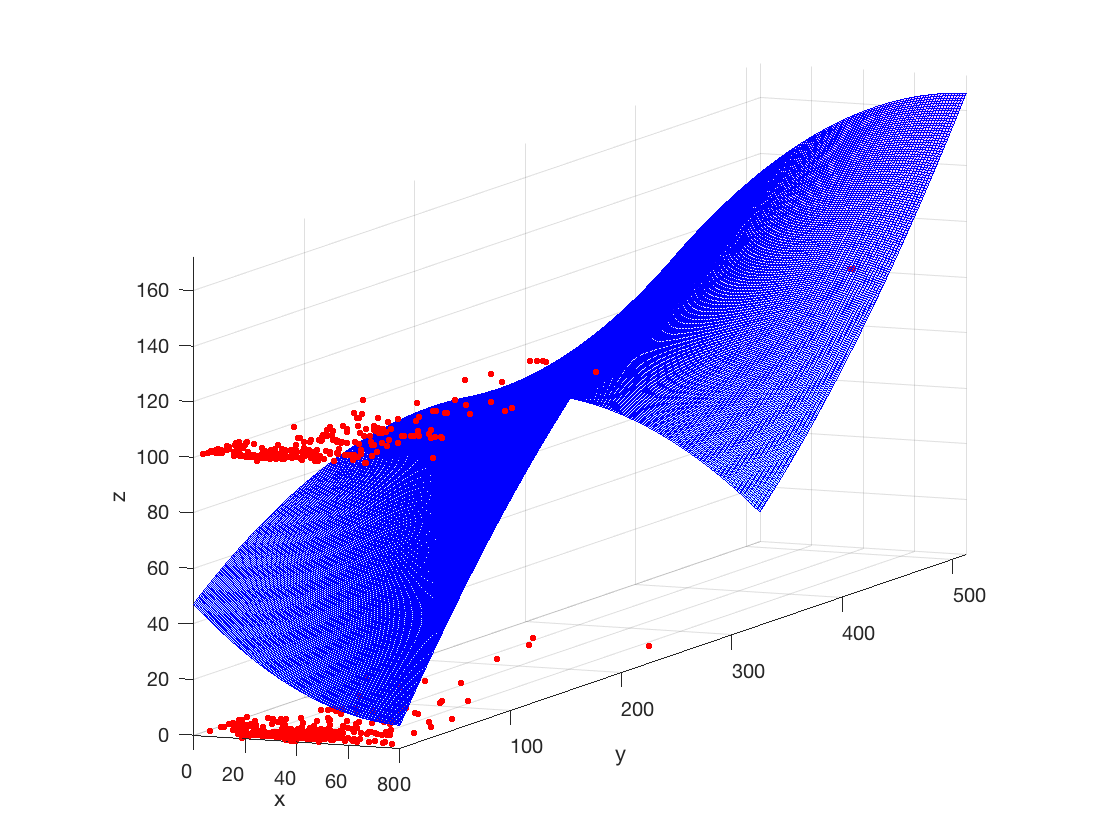
\includegraphics[scale=0.2]{2Dcurve.png}
\end{minipage}%
\begin{minipage}{.5\textwidth}
  \centering
  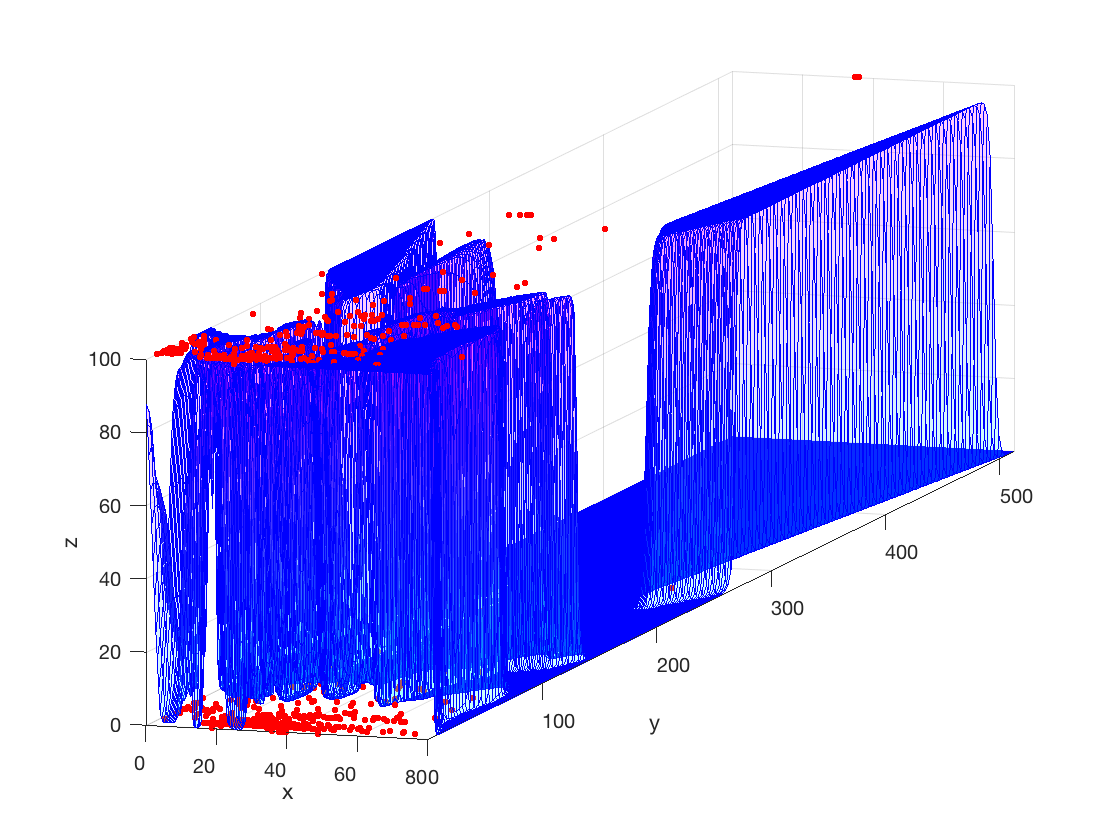
\includegraphics[scale=0.2]{DNN.png}
\end{minipage}
\end{figure}



\end{document}